%%%%%%%%%%%%%%%%%%%%%%%%%%%%%%%%%%%%%%%%%%%%%%%%%%%%%%%%%%%%%%%%%%%%%%%%%%%%%%%
\chapter{Fluidi non newtoniani}\label{chp:NonNewton}
%%%%%%%%%%%%%%%%%%%%%%%%%%%%%%%%%%%%%%%%%%%%%%%%%%%%%%%%%%%%%%%%%%%%%%%%%%%%%%%
I materiali polimerici non possiedono comportamento newtoniano.
Possiamo definire come "newtoniano" un fluido per il quale:
\begin{description}
\item[Fluido newtoniano] la viscosità dipende unicamente da temperatura e pressione: $\eta = \eta(T,p)$
\end{description}

Una prima relazione che lega la viscosità a temperatura e pressione può essere quella di \textit{Arrhenius}:
\begin{equation}
\eta = \eta_t e^{\frac{\Delta E}{R}\left(\frac{1}{T}-\frac{1}{T_0}\right)} %
e^{\beta \left(p - p_0\right)}
\label{eqn:Arrhenius}
\end{equation}
Resta evidente come:
\begin{itemize}
\item Se $p \uparrow\uparrow$ allora $\eta \uparrow\uparrow$.
\item Se $T \uparrow\uparrow$ allora $\eta \downarrow\downarrow$. 
\end{itemize}

Nello specifico, i fluidi non newtoniani presentano delle così dette \textbf{deviazioni} dal comportamento del fluido newtoniano.
Ora verranno elencate e poi approfondite nello stesso ordine.

\begin{enumerate}
\item La viscosità dipende dalle condizioni di flusso, in particolare dalla velocità di deformazione.
\item Possono esserci effetti di sforzo normale.
\item Possono esserci effetti di viscoelasticità.
\item Possono esserci effetti di plasticità: ovvero fenomeni di snervamento.
\item Gli effetti sono conseguenze del tempo: \textbf{tissotropia}.
\end{enumerate}

\section{Condizioni di flusso}
Come accennato in precedenza, una deviazione dal comportamento di fluido newtoniano può essere quella della dipendenza dalle condizioni di flusso alle quali il fluido viene sottoposto.
In particolare i fluidi non newtoniani dipendono fortemente dalla velocità di deformazione $\dot{\gamma}$.
Perciò, vale:
\begin{equation}
\eta = \eta(\dot{\gamma})
\label{eqn:viscNonNewt}
\end{equation}
Funzione che lega la viscosità con la velocità di deformazione.
Siccome lo \textbf{sforzo di taglio} vale, sia per fluidi newtoniani che non:
\begin{equation}
\tau = \eta \dot{\gamma}
\label{eqn:sforzoTaglio}
\end{equation}
Da cui, sostituendo la \eqref{eqn:viscNonNewt} alla \eqref{eqn:sforzoTaglio} ne risulta:
\begin{equation}
\tau = \eta(\dot{\gamma}) \dot{\gamma}
\label{eqn:taglioNonNewt}
\end{equation}

\begin{figure}
\centering
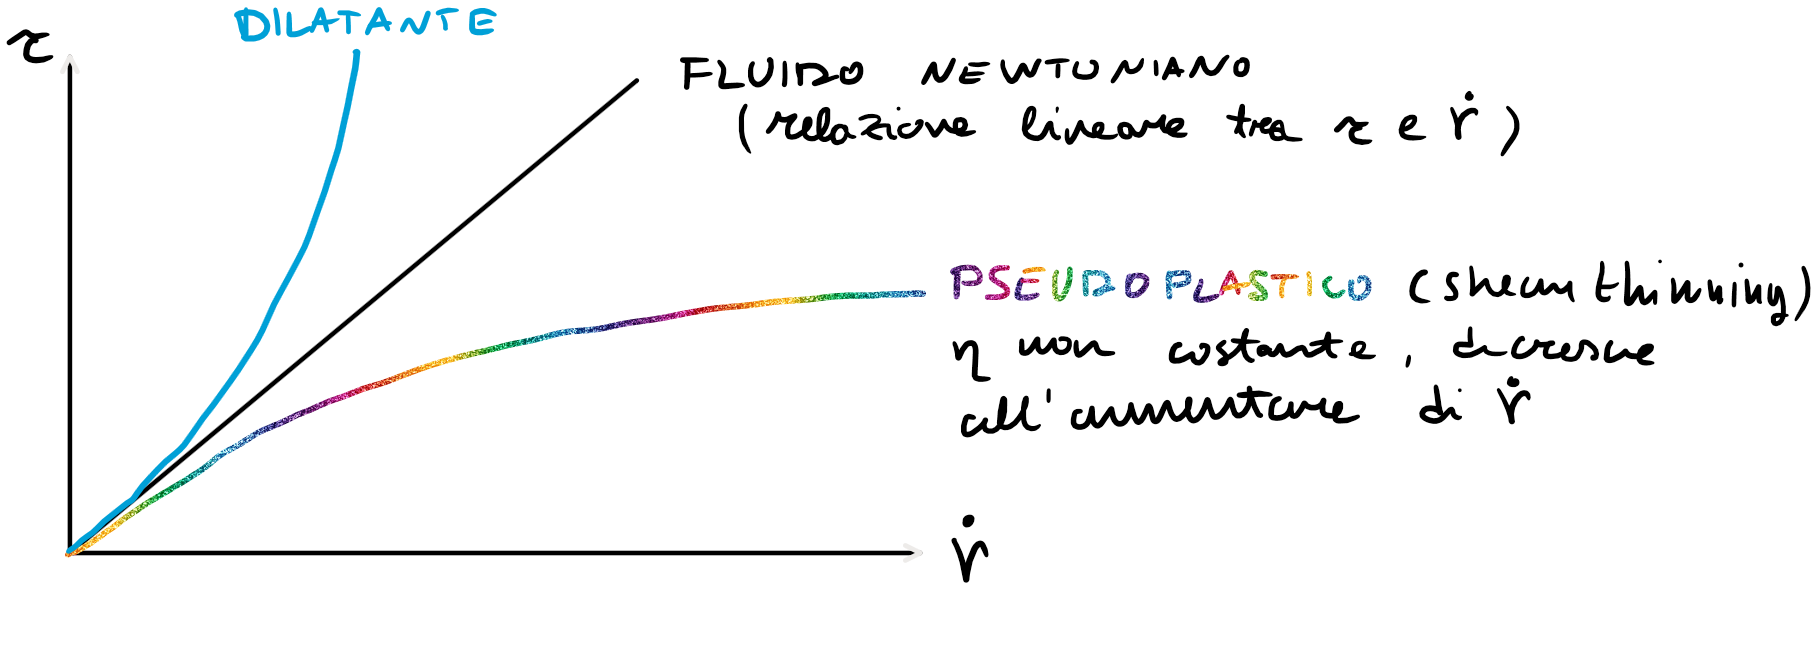
\includegraphics[width = \textwidth]{gfx/TaglioNonNewt}
\caption{Andamento dello sforzo di taglio per diversi fluidi}
\label{fig:TaglioNonNewt}
\end{figure}

Dal grafico \ref{fig:TaglioNonNewt} si può dedurre che:
all'aumentare dello sforzo di taglio il fluido si assottiglia (cioè ha comportamento \textbf{pseudo-plastico} e $\eta$ diminuisce).
Quasi tutti i materiali plastici hanno comportamento pseudo-plastico. Con $\eta$ indipendente dal tempo.
Se $\dot{\gamma}$ aumenta, significa che il fluido di assottiglia sempre di più perché viene speso molto sforzo di taglio per deformare l'oggetto. In generale viene considerato un vantaggio.

Per un fluido polimerico, si può tracciare un comportamento del tipo \ref{fig:PesudoPlastico}.

\begin{figure}
\centering
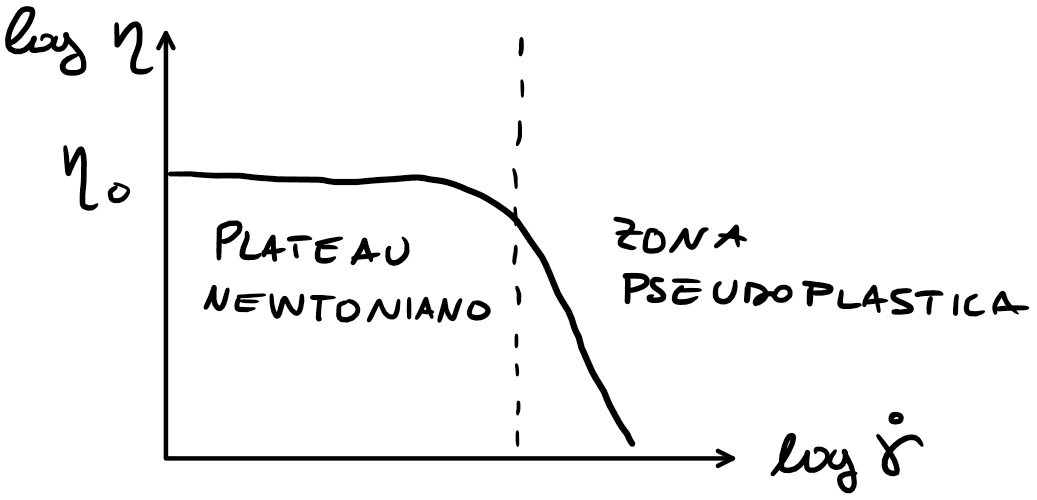
\includegraphics[width = 0.7\textwidth]{gfx/PseudoPlastico}
\caption{Comportamento di un fluido polimerico}
\label{fig:PesudoPlastico}
\end{figure}

\section{Effetti di sforzo normale e viscoelasticità}
\subsection{Sforzo normale}
Se al fluido, all'interno di un qualsiasi contenitore, viene applicato uno sforzo esterno, questo risale grazie ad un movimento di rotazione circonferenziale provocato dall'aderenza.
A livello circonferenziale, le catene polimeriche sono sollecitate a trazione. Tuttavia, nel corso del tempo esse tenderanno a ritornare allo stadio iniziale di gomitolo statistico, esercitando una pressione sull'elemento rotante. Creando così aderenza.
Questo viene anche chiamato \textbf{effetto Poisson}.

\subsection{Viscoelasticità}
Viene detto \textbf{effetto Barus} o di \textbf{rigonfiamento dell'estruso}.
Vengono rappresentati nei grafici \ref{fig:RigonfiamentoEstruso}.

\begin{figure}
\centering
\subfloat[][\emph{Effetto di rigonfiamento dell'estruso}\label{fig:Barus}]
{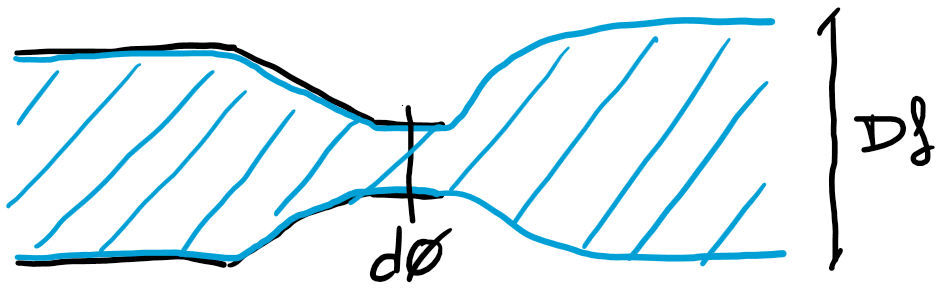
\includegraphics[width = 0.4\textwidth]{gfx/Barus}}\quad
\subfloat[][\emph{Comportamento per fluidi con effeto di rigonfiamento a diverso comportamento elastico}\label{fig:Elasticità}]
{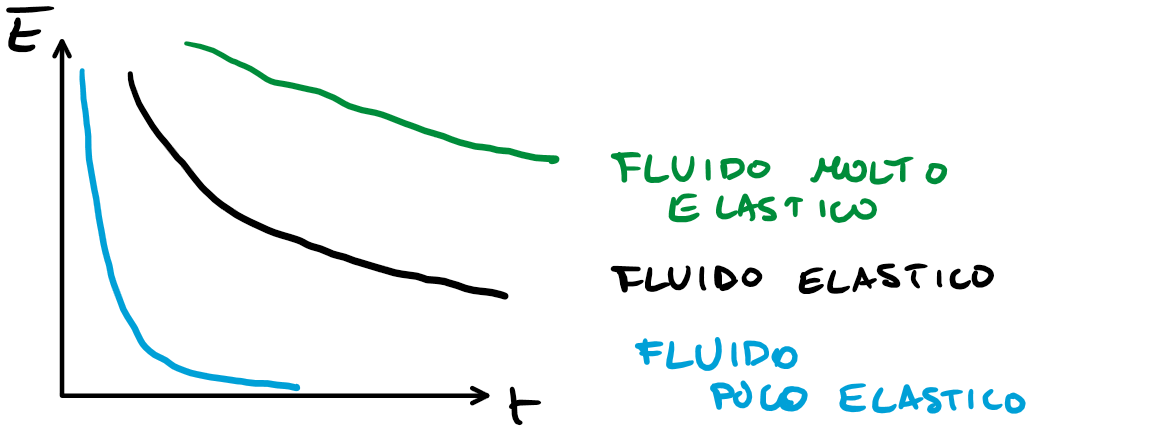
\includegraphics[width = 0.4\textwidth]{gfx/Elasticità}}
\caption{Comportamento dei fluidi con effetto di rigonfiamento dell'estruso}
\label{fig:RigonfiamentoEstruso}
\end{figure}

Si definisce che l'effetto di rigonfiamento:
\begin{equation}
De = \frac{\tau_r}{\tau_p} = \frac{\text{Tempo di rilassamento}}{\text{Tempo caratteristico del processo}}
\end{equation}
Da cui ne deriva:
\begin{description}
\item[$\tau_r \ll \tau_p$] allora $De \approx 0$ allora si dice che il fluido è poco elastico. Comportamento evidenziato al grafico \ref{fig:Elasticità}.
\item[$\tau_r \approx \tau_p$] allora $De \approx 1$ allora si dice che il fluido è più elastico. Sempre evidenziato al grafico \ref{fig:Elasticità}.
\end{description}

\section{Effetti di plasticità}
Un fluido pseudo-plastico possiede forze interne (intermolecolari) che che gli conferiscono il moto al di sotto di un certo valore $\tau$, il fluido non muoverà fino a quando tale valore non verrà superato (Comportamento del fluido di \textbf{Bingham}). 
Sotto lo \eng{Yield stress} il fluido si comporta come solido.
Sopra lo \eng{Yield stress}, lo sforzo cresce con $\dot{\gamma}$.

Il grafico \ref{fig:EffettoPlastico} rappresenta i comportamenti di un fluido puramente pseudo-plastico e il fluido di Bingham.
Entrambi hanno una legge del tipo:
\begin{description}
\item[Fluido di Bingham] $\tau = \tau_y + \eta \dot{\gamma}$
\item[Fluido pseudo-plastico] $\tau = \eta \dot{\gamma}$
\end{description}

\begin{figure}
\centering
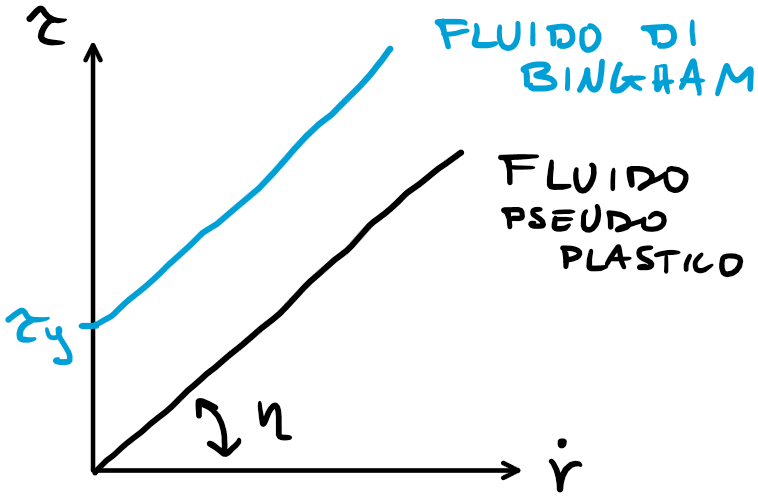
\includegraphics[width = 0.6\textwidth]{gfx/EffettoPlastico}
\caption{Rappresentazione del comportamento sotto l'effetto plastico}
\label{fig:EffettoPlastico}
\end{figure}

\section{Tissotropia}
\begin{figure}
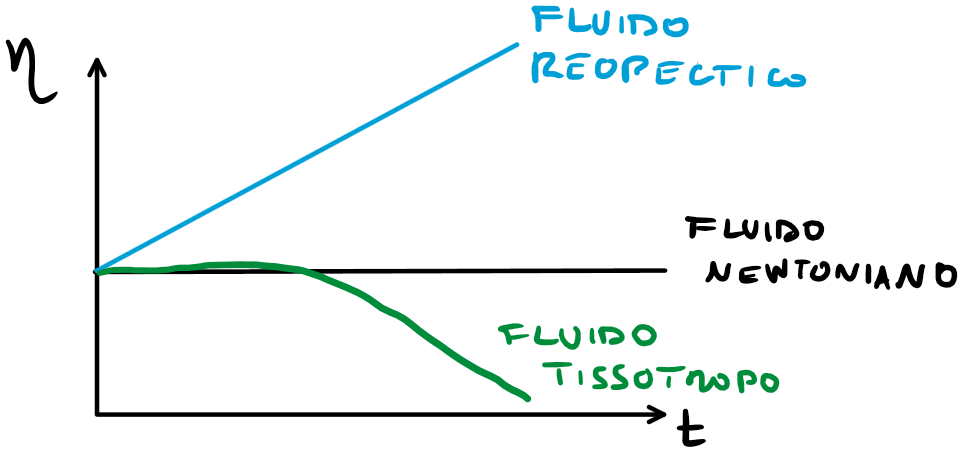
\includegraphics[width = 0.7\textwidth]{gfx/Tissotropia}
\caption{Caratteristica della viscosità in funzione del tempo}
\label{fig:Tissotropia}
\end{figure}
La tissotropia si può presentare in due forme particolari:
\begin{description}
\item[Fluido reopectico] sono quei (pochi) fluidi che aumentano la loro viscosità all'aumentare del tempo.
\item[Fluido tissotropico] sono i fluidi, non newtoniani che diminuiscono la loro viscosità all'aumentare del tempo.
\end{description}

%%%%%%%%%%%%%%%%%%%%%%%%%%%%%%%%%%%%%%%%%%%%%%%%%%%%%%%%%%%%%%%%%%%%%%%%%%%%%%%
\chapter{Reologia (o Reometria)}\label{chp:Reologia}
%%%%%%%%%%%%%%%%%%%%%%%%%%%%%%%%%%%%%%%%%%%%%%%%%%%%%%%%%%%%%%%%%%%%%%%%%%%%%%%
La reologia studia la deformazione di un corpo sotto l'azione di uno sforzo.
I fluidi ideali, liquidi o gassosi che siano, si deformano irreversibilmente. L'energia di deformazione viene dissipata all'interno dei fluido sotto forma di calore, non può essere recuperata alla cessazione dello sforzo. Nella realtà non si trovano né fluidi ideali, né solidi ideali.
Solo pochi liquidi si avvicinano, come comportamento a quello dei liquidi ideali. La maggior parte dei liquidi mostrano reologiacamente un comportamento che li classifica nella regione tra i liquidi e solidi: essi sono sia elastici che viscosi e possono perciò essere definiti "viscoelastici", che possono subire solo sforzi di taglio.

La resistenza di un fluido rispetto ad ogni cambiamento irreversibile dei suoi elementi di volume viene detta viscosità.

\section{La legge della viscosità}
\subsection{La legge di Newton}
LA misura della viscosità dei liquidi richiede dapprima la definizione dei parametri che riguardano il flusso. Si potranno poi trovare opportune condizioni per l'esecuzione dei test che consentono la misurazione delle grandezze in modo obbiettivo e riproducibile.
Newton fu il primo a formulare la legge fondamentale della viscometria che descrive il comportamento di flusso di un liquido ideale.
\begin{equation}
\tau = \eta \cdot \dot{\gamma}
\label{eqn:1LeggeNewton}
\end{equation}

\paragraph{Lo sforzo di taglio}
Una forza $\mathbf{F}$ applicata ad un'area $A$ (interfaccia tra il piatto superiore il il liquido sottostante) provoca un movimento di scorrimento nello strato liquido. la velocità di flusso che può essere mantenuta per una data forza sarà determinata dalla resistenza interna del liquido, cioè dalla sua viscosità.
\begin{equation}
p = \frac{\mathbf{F}}{A} = \left[\frac{N}{m^2}\right] = \left[Pa\right]
\end{equation}

\section{Le curve di flusso e di viscosità}
la correlazione tra lo sforzo di taglio e gradiente di velocità che definisce il comportamento reologico di un liquido può essere graficamente riportato in un diagramma $t/D$. Il diagramma prende il nome di \textbf{curva di flusso}.
Altro diagramma assai comune è quello che riporta $\eta$ in funzione di $D$ (velocità). Questo diagramma è detto \textbf{Curva di viscosità}.